% Beamer's default font size is 11 points. It is possible to set the
% default font size to any of 8, 9, 10, 11, 12, 14, 17, 20
\documentclass[13pt]{beamer}

\usetheme{Warsaw}
%\usecolortheme{dolphin}
\usecolortheme{seahorse}
%\useinnertheme{circles}
\usefonttheme{professionalfonts}
%\usefonttheme{structurebold}
%\usefonttheme{default}

\setbeamertemplate{navigation symbols}{}
 
\usepackage[english]{babel}
\usepackage[latin1]{inputenc}
\usepackage{times}
\usepackage[T1]{fontenc}
\usepackage{fancybox}
\usepackage{floatflt}


% These things can change:
\newcommand{\baseurl}{http://cell.vtt.fi/latex}
\urlstyle{sf}
\newcommand{\plus}{\makebox[2em]{+}}
\newcommand{\minus}{\makebox[2em]{-}}

% In beamer, defining new commands inside the slides fails.
\newcommand{\warning}[1]{%
\begin{center}
\Large
\shadowbox{
\textbf{#1}}
\end{center}
}

\begin{document}

\logo{
\includegraphics[width=1.4cm]{img/vttplain}\quad}
\title{\scalebox{1.5}{\textrm{\LaTeX}} Course 2011}
\subtitle{Part 5: Graphics}
\author{Arho Virkki}
\institute{\textsc{VTT Technical Research Centre of Finland}}
\date{\scalebox{0.8}{\textcolor{gray}{}}}

\begin{frame}[fragile]
  \titlepage
\end{frame}

\begin{frame}[fragile]\frametitle{Adding images}
Adding images to text became a routine task around the beginning of 
1990's.\footnote{At least to what the author can remember from those
early days of computing e.g. without stuff like Internet.}\medskip

Because of this, the commands to handle graphics are loaded separately 
to \LaTeX{} even today:
\begin{verbatim}
\usepackage{graphicx}
\usepackage{color}
\end{verbatim}
or
\begin{verbatim}
\usepackage{graphicx,color}
\end{verbatim}
\end{frame}


\begin{frame}[fragile]\frametitle{Adding images...}
A simple example:
\begin{verbatim}

\includegraphics{img/foo}
\end{verbatim}

\includegraphics{img/foo}
\end{frame}


\begin{frame}[fragile]\frametitle{Adding images...}
\begin{itemize}
\item \verb|\includegraphics{file_with_no_extension}|
adds an image to the document
\item The extension of the file (.eps, .pdf, .png, .jpg) was intentionally left
out: The compiler (e.g. \texttt{latex} or \texttt{pdflatex}) will choose the
file with the correct extension on its own. 
\item Writing the extension explicitly will force the selection
(and cause an error on certain cases:
\begin{itemize}
\item The traditional \LaTeX{} understands only the \texttt{.eps} files
\item PDF\LaTeX{} can read \texttt{.pdf}, \texttt{.png} and \texttt{.jpg} 
  files, but \textbf{not} the \texttt{.eps} files $\Rightarrow$ 
  brilliant!\dots
\end{itemize}
\end{itemize}
\end{frame}


\begin{frame}[fragile]\frametitle{Adding images...}
Changing the format between 
\[ \text{\texttt{.pdf}} \leftrightarrow
   \text{\texttt{.eps}} \leftrightarrow
   \text{\texttt{.png}} \leftrightarrow
   \text{\texttt{.jpg}} \]
is nevertheless easy.
\begin{itemize}  
\item In unix, the work can be done with the commands
\texttt{epstopdf} or \texttt{pdftops}\footnote{The conversion between the 2005
and 2011 LaTeX course graphics files (including several eps illustrations) was
done in command line with the single loop: \texttt{for f in *eps; do epstopdf \$f;
done}\\ \strut} or using
\item the GIMP or ImageMagic programs (freely available for Windows, Linux and
Mac).
\end{itemize}
\end{frame}


\begin{frame}[fragile]\frametitle{Adding images...}
By default, the image files are searched from the same folder where the
manuscript resides. If there are plenty of images, it might be a good option
to store them on a separate sub-folder. In this case, the images must be linked
with 
\begin{itemize}
\item the relative path \verb|
\includegraphics{image_path/foo}| or
\item using the command \verb|\graphicspath{{}{}...{}}|
\end{itemize}
Example:
\begin{verbatim}
\graphicspath{{/home/arho/images/}
              {images/}}

\includegraphics{images/foo}
\end{verbatim}
\end{frame}


\begin{frame}[fragile]
\frametitle{\texttt{$\boldsymbol{\backslash}$includegraphics[]\{\}}}
\verb|\includegraphics| accepts quite a number of optional key-value parameters.
For example:
\begin{verbatim}

\includegraphics[width=0.3\textwidth,
                 angle=45]{img/foo}
\end{verbatim}

\includegraphics[width=0.3\textwidth,
                 angle=45]{img/foo}
\end{frame}


\begin{frame}[fragile]
\frametitle{\texttt{$\boldsymbol{\backslash}$includegraphics[]\{\}...}}
The most common optional parameters include:\medskip
\begin{itemize}
\item \verb|scale=number| scaling the image as compared to the original
\item \verb|width=length| setting the width 
\item \verb|height=lenght| setting the height
\item \verb|angle=degrees| turning the image counterclockwise (=to the positive
direction in the mathematical sense) \end{itemize}\medskip
\begin{flushleft}
Note! The lenght must incorporate the unit, e.g. \verb|1.5cm| or
\verb|0.2\textwidth| and the scaling factors are with no units.
\end{flushleft}
\end{frame}


\begin{frame}[fragile]\frametitle{Figure environments}
Sometimes, adding the images to the proper position can be left to the computer,
and it is always a good idea to let the machine to keep record of the
actual image number. Example:
\begin{verbatim}
\begin{figure}[!htbp]
\begin{center}

\includegraphics[width=0.4\textwidth]{img/foo}
\caption{A schematic illustration of the Gadget}
\label{fg:foo}
\end{center}
\end{figure}
\end{verbatim}
\end{frame}


\begin{frame}[fragile]\frametitle{Figure environments...}
\begin{figure}[!htbp]
\begin{center}

\includegraphics[width=0.4\textwidth]{img/foo}
\caption{A schematic illustration of the Gadget}
\label{fg:foo}
\end{center}
\end{figure}
The image can be cited later with  \verb|\ref{fg:foo}| (which will be replaced
with the actual image number in the compiled document).
\end{frame}


\begin{frame}[fragile]\frametitle{Figure environments...}
The optional parameter \verb|[!htbp]| means, that
\begin{itemize}
\item I really would like(\textbf{!}) to insert
\item the picture right \textbf{h}ere or, if not,
\item to the \textbf{t}op or
\item to the \textbf{b}ottom of this page and,
\item if this also fails, to a separate
\textbf{p}icture page.
\end{itemize}
\end{frame}


\begin{frame}[fragile]\frametitle{Figure environments...}
There exists an additional package \texttt{floatflt} for making the text to
surround the
images\footnote{Apparenty there are some issues with the freedom\\ of the 
license of this package, but it can be installed by hand {\tiny
\url{http://blogs.fau.de/johanneshabich/2010/05/20/latex-floatflt-sty-missing-on-ubuntu-lucid-10-04/}}}

\small
\begin{verbatim}
\begin{floatingfigure}{4cm}

\includegraphics[width=3cm]{img/foo}
\caption{StarBox3D}
\label{fg:fooii}
\end{floatingfigure}
By inspecting the figure, we see that the optimal 
decision threshold for separating the control and 
positive classes is obviously at $b$, where also
the conditional probability $p(P|b)=0.5$. However,... 
\end{verbatim}
\end{frame}

\begin{frame}[fragile]\frametitle{Figure environments...}
\begin{floatingfigure}{4cm}

\includegraphics[width=3cm]{img/foo}
\caption{StarBox3D}
\label{fg:fooii}
\end{floatingfigure}
By inspecting the figure, we see that the optimal 
decision threshold for separating the control and 
positive classes is obviously at $b$, where also
the conditional probability $p(P|b)=0.5$. However,...
\end{frame}


\begin{frame}[fragile]\frametitle{Colors}
Colors are easiest to add with the package
\begin{verbatim}
\usepackage{color}
\end{verbatim}
but the number of colors is rather limited --- {\small but should at least
include white, black, red, green, blue, cyan, magenta and yellow\footnote{%
\url{http://en.wikibooks.org/wiki/LaTeX/Colors}\\[0.5ex]}}. To define a
custom color, we need the additional command

\begin{verbatim}
\definecolor{col_name}{col_system}{col_def}
\end{verbatim}
For example
\begin{verbatim}
\definecolor{mygreen}{rgb}{0.61,0.78,0.05}
\colorbox{vihrea}{Nice Green Backround!}
\end{verbatim}
\definecolor{mygreen}{rgb}{0.61,0.78,0.05}
\colorbox{mygreen}{Nice Green Backround!}
\end{frame}


\begin{frame}[fragile]\frametitle{Colors...}

Using the pre-defined colors is easy
\begin{verbatim}
\colorbox{orange}{Orange}
\fcolorbox{red}{green}{Pearl}
\textcolor{blue}{
\[ \sum_{k=1}^\infty a_k \]}
\end{verbatim}
\colorbox{orange}{Orange}
\fcolorbox{red}{green}{Pearl}
\textcolor{blue}{
  \[ \sum_{k=1}^\infty a_k \]}
\end{frame}

\begin{frame}[fragile]\frametitle{Using \LaTeX{} to draw images}
\LaTeX{} has a built-in system to draw simple images. The following example is
from the book of Kopka and Daly.
\begin{verbatim}
\setlength{\unitlength}{0.8cm}
\begin{picture}(5,2)\thicklines
  \put(5,0){\vector(-1,0){5}}
  \put(0,0){\vector(1,1){2}}
  \put(2,2){\vector(3,-2){3}}
\end{picture}
\end{verbatim}
\begin{center}
\setlength{\unitlength}{0.8cm}
\begin{picture}(5,2)\thicklines
  \put(5,0){\vector(-1,0){5}}
  \put(0,0){\vector(1,1){2}}
  \put(2,2){\vector(3,-2){3}}
\end{picture}
\end{center}
\end{frame}


\begin{frame}[fragile]\frametitle{Drawing images...}
For a comparison, some PostScript code\footnote{PostScript is nowadays
superseded by the pdf format\\ \strut} (again from K\&D):
\begin{verbatim}
%!PS-Adobe-3.0 EPSF-3.0
%%BoundingBox: 169 158 233 242
220 200 moveto
200 200 20 0 360 arc
170 170 moveto
230 220 lineto
170 210 lineto
225 160 lineto
205 240 lineto
170 170 lineto
stroke
showpage
\end{verbatim}
\end{frame}


\begin{frame}[fragile]\frametitle{Drawing images...}
This code produces the image
\begin{center}
\includegraphics[width=0.3\textwidth]{img/hassakka}
\end{center}
The following example is a bit more complicated\dots
\end{frame}


\begin{frame}[fragile]\frametitle{Drawing images...}
\small
\begin{verbatim}
%!ps
/iter 60 def /reso .005 def /sq { dup mul } def
/mod { 2 copy div floor mul sub } def /plot {
newpath moveto 1 0 rlineto stroke } def gsave
280 420 translate 260 2 div dup scale 2 260 div
setlinewidth -2 reso 2 { /x exch def -2 reso 2 {
/y exch def /r 0 def /i 0 def /n 0 def iter { r
sq i sq add 4 gt { exit } if /rr r sq i sq sub x
add def /i 2 r mul i mul y add def /r rr def /n
n 1 add def } repeat n 10 mod .1 mul .1 add
setgray x y plot } for } for grestore showpage
\end{verbatim}
\end{frame}


\begin{frame}[fragile]\frametitle{Drawing images...}
\begin{center}

\includegraphics[width=0.7\textwidth]{img/mandelbrot}
\end{center}
\end{frame}


\begin{frame}[fragile]\frametitle{Drawing images...}
\begin{itemize}
\item The command languages are precise, because the images are not stored as
pixels, but as lines, circles, B\'ezier curves,\ldots, and text (with the
corresponding size and font).
\item For some purposes, using svg or similar language might be beneficial.
\item The LaTeX default language is rather poor, as e.g. the angles of the line
can only have some fixed values
\item A better investment for a casual used is to learn a drawing tool (e.g.
Inkscape\footnote{\url{http://inkscape.org/}} for vector graphics or
Gimp\footnote{\url{http://www.gimp.org}} for digital photographs)
\end{itemize}
\end{frame}


\begin{frame}[fragile]\frametitle{Drawing images...}
Which program to use? The answer depend on the personal taste (as well as the
willingness to pay for commercial software). Nevertheless, if we restrict
ourselves only to the free options, 

\begin{itemize}
\item GIMP is the choice for painting (pixel map images like digital photos)
\item Inkscape is the choice for vector graphics (where e.g. the circles are
truly Platonian, and the device (= printer or screen) only does its best to
approximate the idea)
\item Programming environments like R, Matlab and gnuplot all produce
high-quality plots in pdf format (which can be further polished with Inkscape,
if desired).
\end{itemize}
\end{frame}


\begin{frame}[fragile]\frametitle{Drawing images...}
Gimp is purely a program for painting (bitmap images, including digital 
photographs and scanned text pages)
\begin{center}
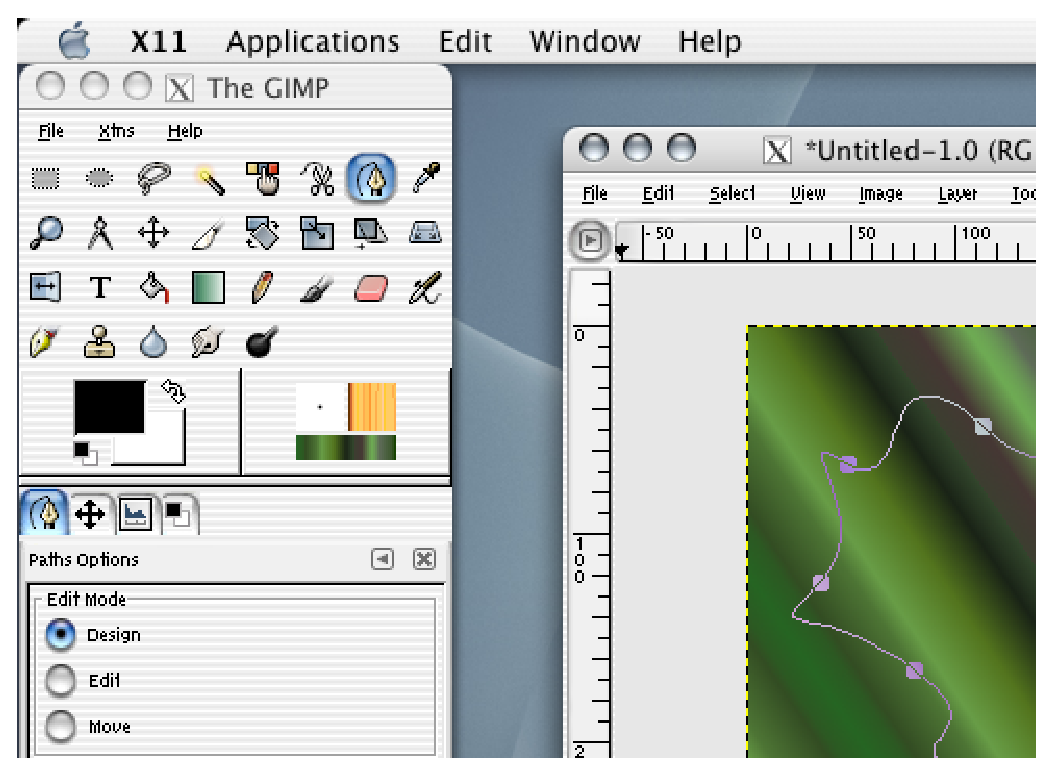
\includegraphics[width=0.7\textwidth]{img/gimpmac}
\end{center}
\end{frame}

\begin{frame}[fragile]\frametitle{Drawing images...}
Inkscape is for vector graphics and resembles the CorelDraw! software
(originated at the early 90's)
\begin{center}
\includegraphics[width=0.8\textwidth]{img/Inkscape}
\end{center}
\end{frame}



\begin{frame}[fragile]\frametitle{Drawing images...}
\small Xfig has not been much updated since 2002 (and the latest change is from
2007) but some people are so used to it, that the program can still be found 
e.g. from the default Debian repositories (and has also been ported to 
Mac OS~X).
\begin{center}
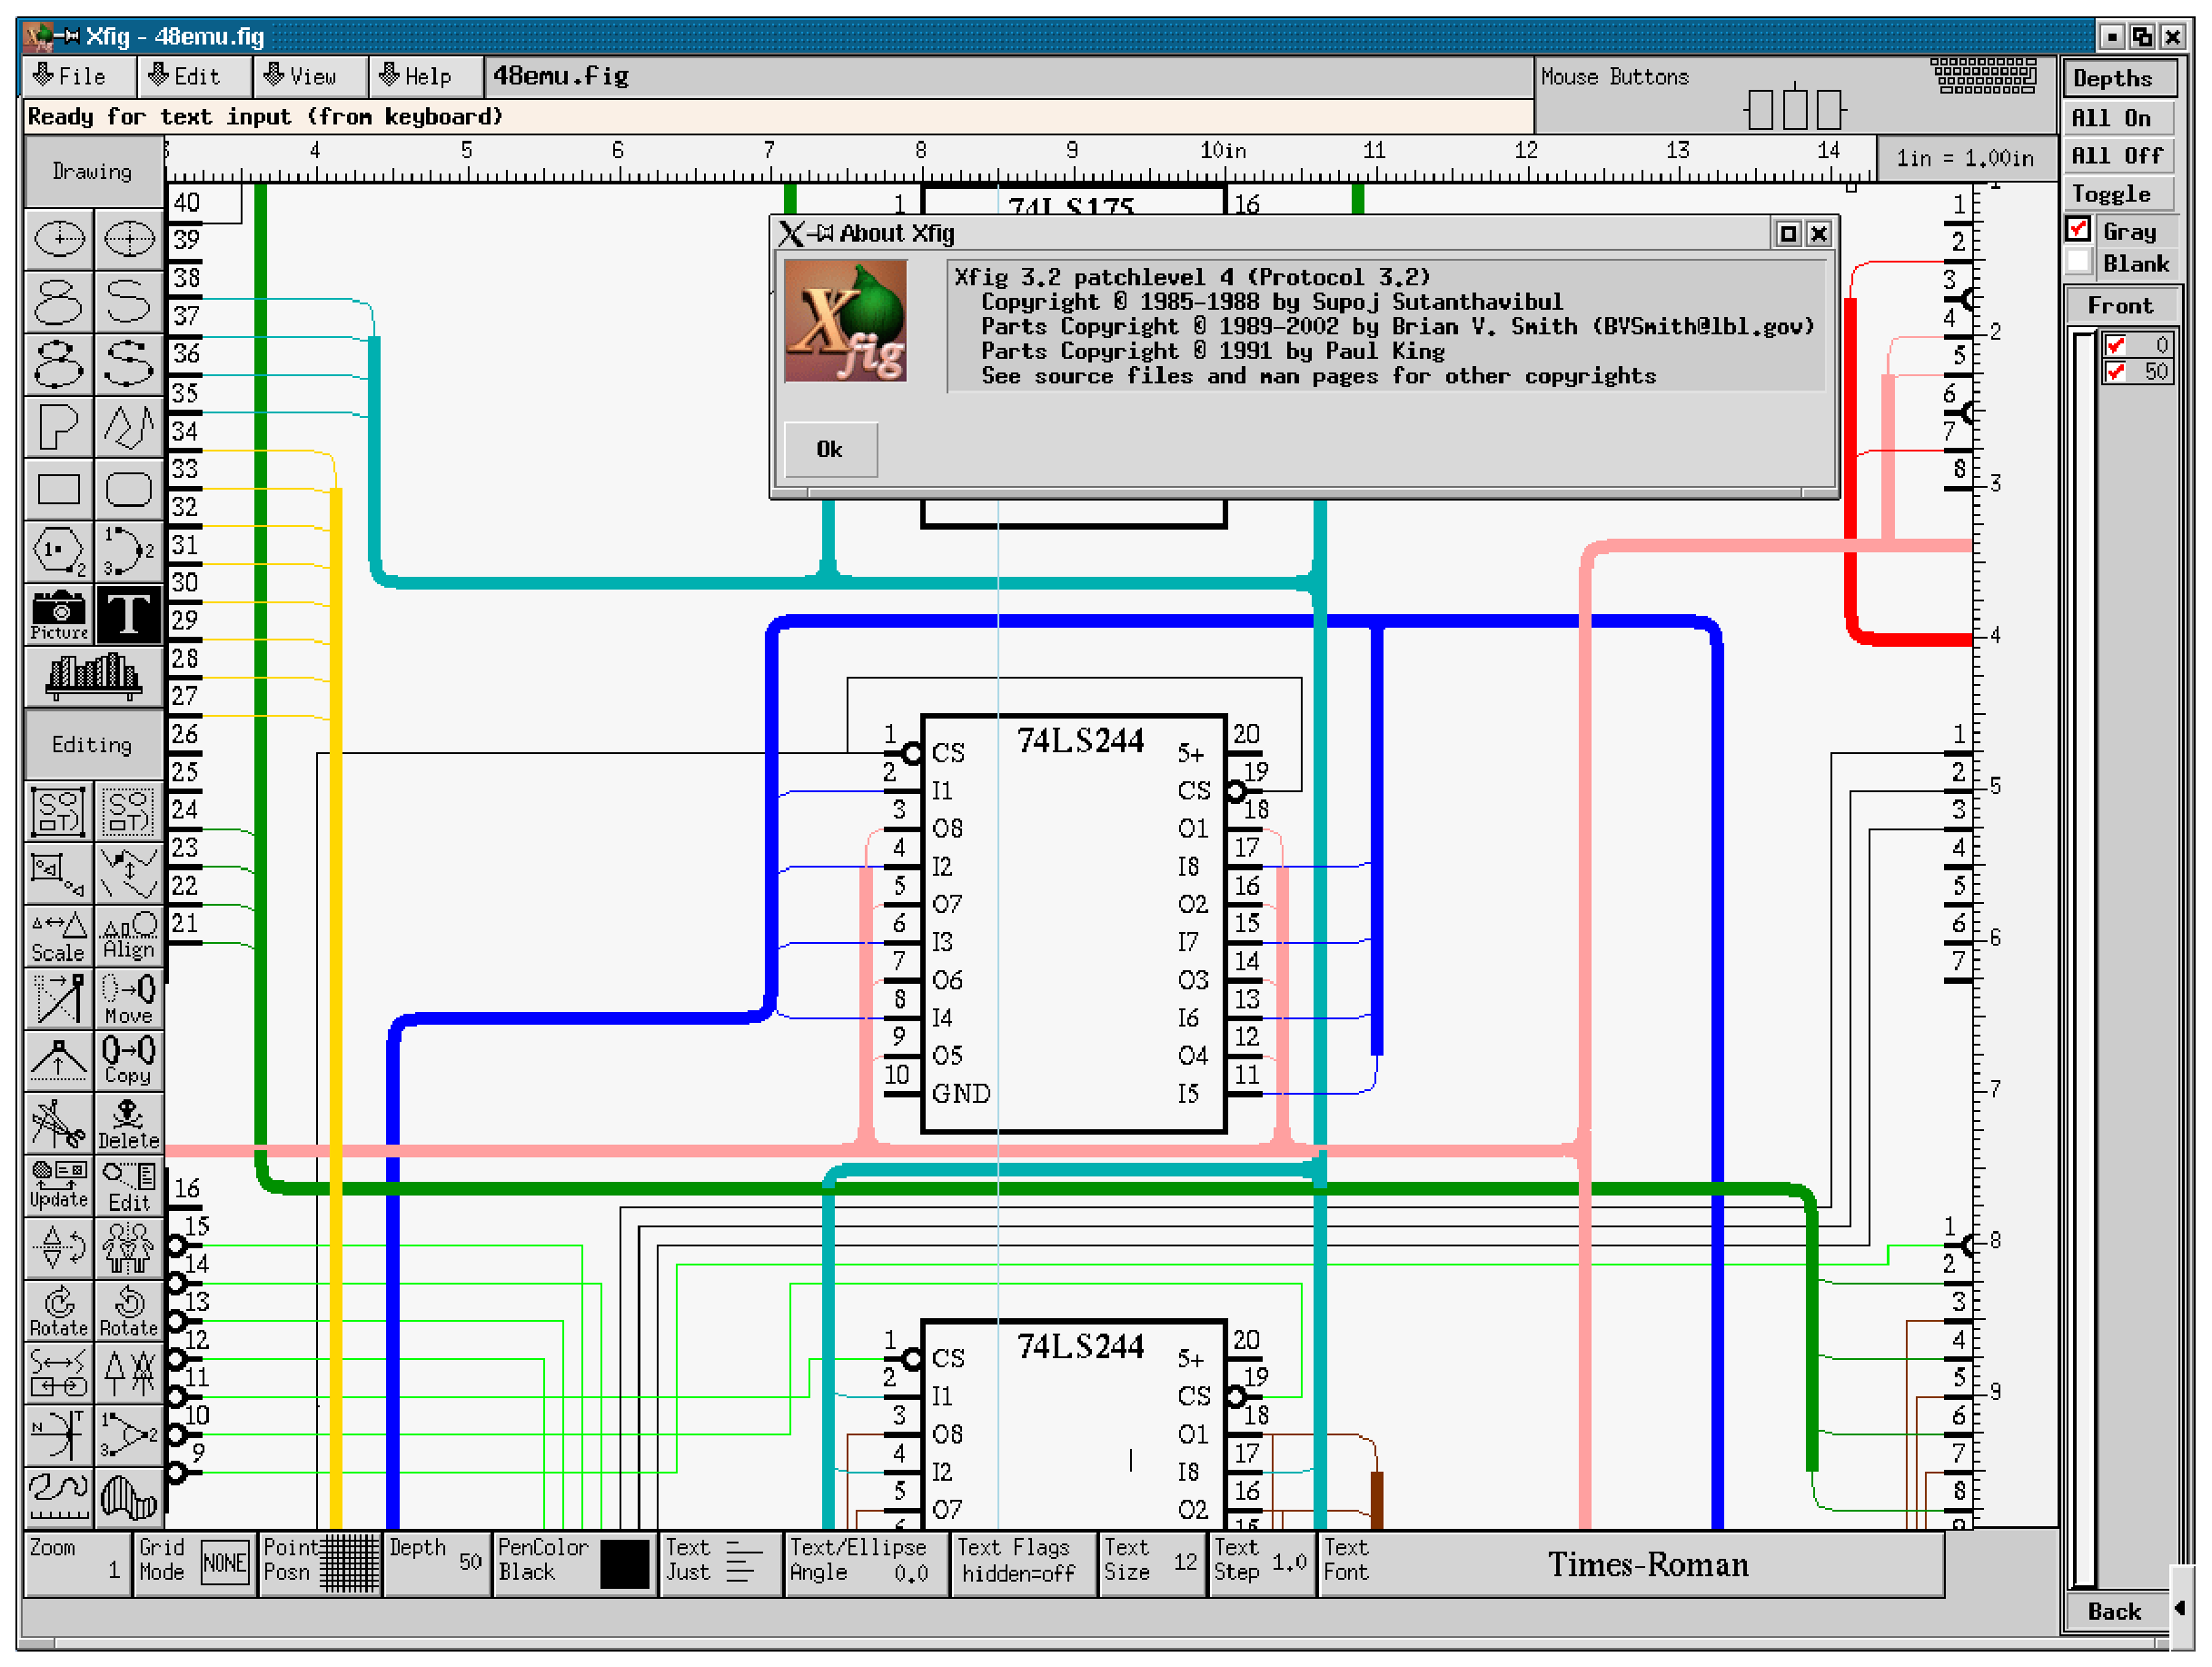
\includegraphics[width=0.62\textwidth]{img/xfig}
\end{center}
\end{frame}


\begin{frame}[fragile]\frametitle{Drawing images...}
\texttt{gnuplot} is yet another ``traditional tool''\footnote{Observe that
all these ``obsolete'' tools are younger than LaTeX\ldots} which uses
its own command language\footnote{\texttt{set pm3d} refers to the OS/2
presentation manager.}
\begin{verbatim}
set pm3d
set contour base
set xrange [-5:5]
set yrange [-5:5]
set isosamples 20,20
set xlabel "x"
set ylabel "y"
unset key
set term post eps enhanced
set output "gnuplotex.eps"
splot x**2-2*y**2 + 2*y -2
\end{verbatim}
\end{frame}


\begin{frame}[fragile]\frametitle{Drawing images...}
The previous code produces the image\\[-2ex]
\hspace*{-1cm}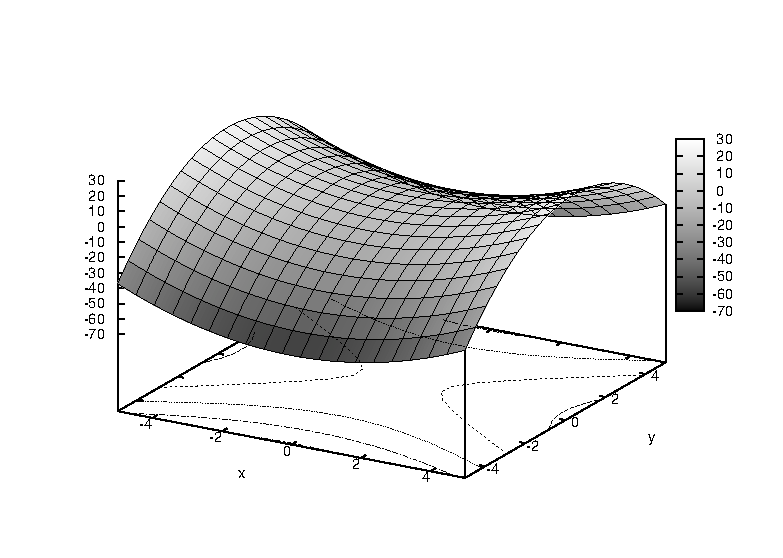
\includegraphics[width=1.1\textwidth]{img/gnuplotex}
\end{frame}


\begin{frame}[fragile]\frametitle{Drawing images...}
The R language and environment for statistical 
computing\footnote{\url{http://www.r-project.org/}}
is an excellent choice for drawing statistical images
\begin{center}
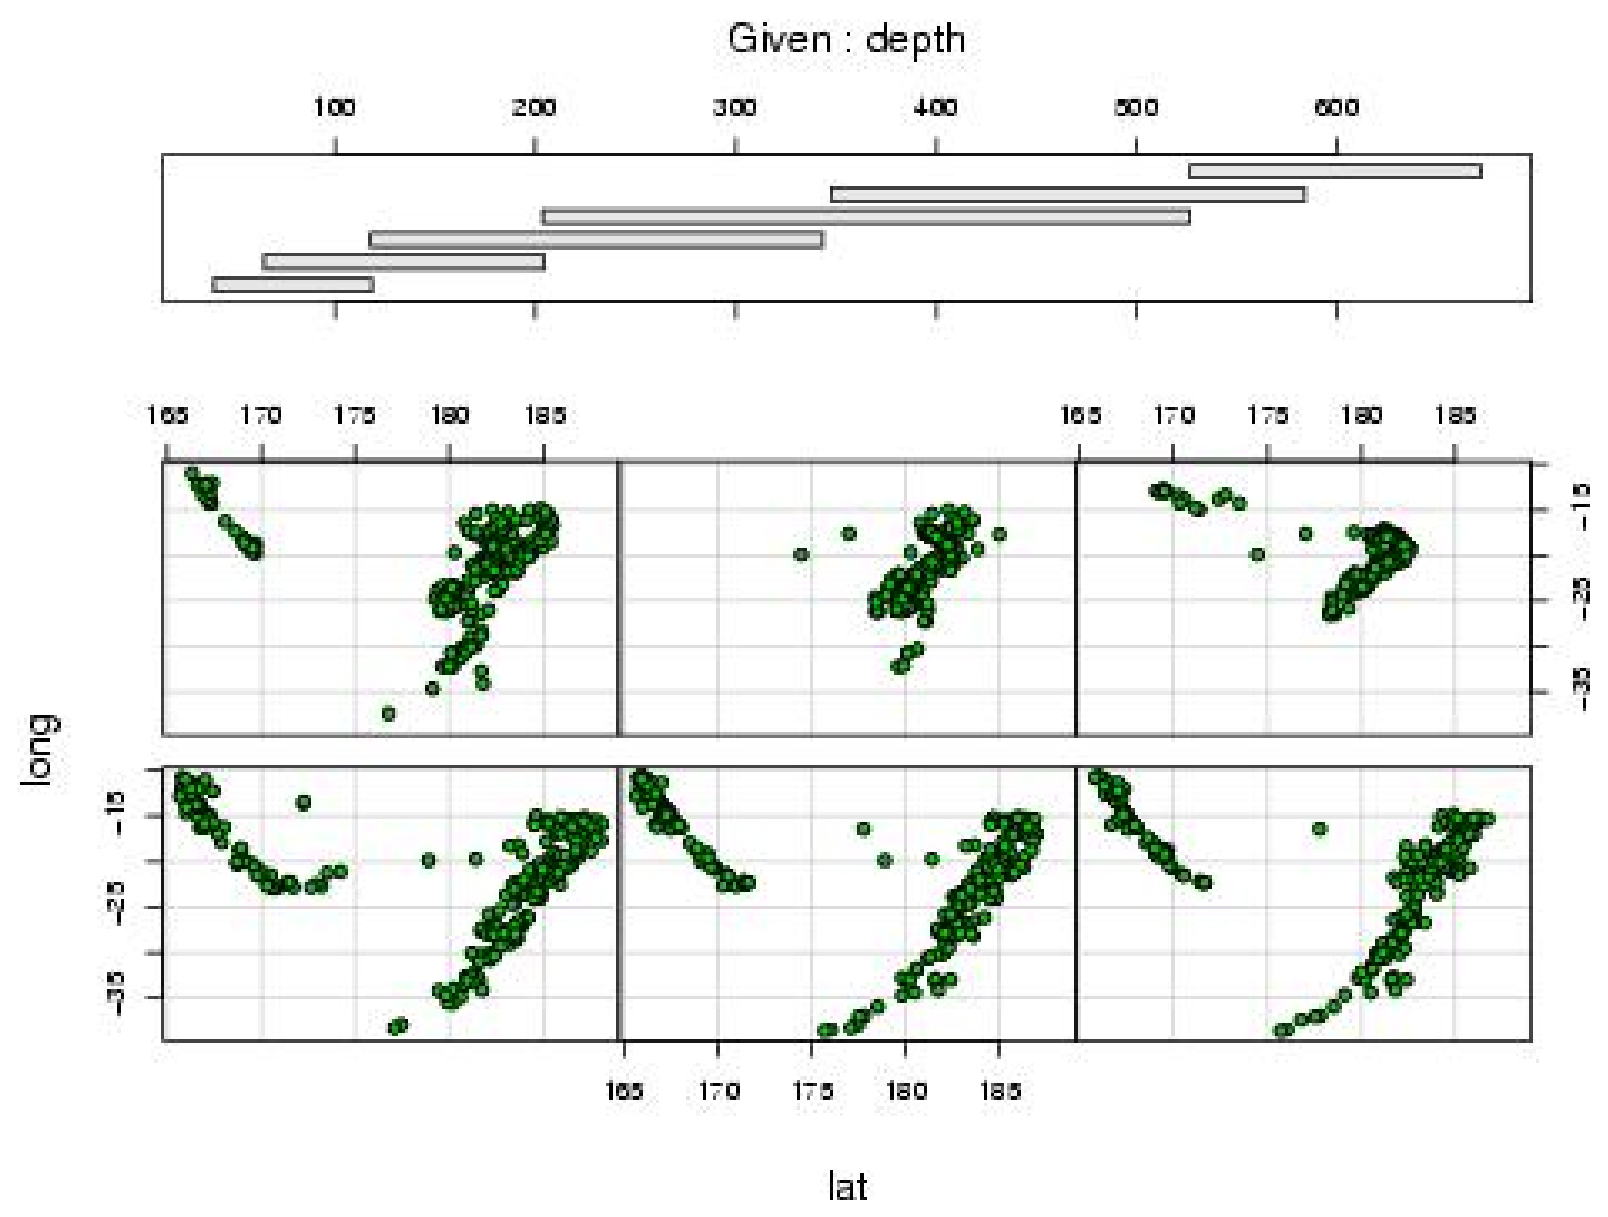
\includegraphics[width=0.7\textwidth]{img/quakes-coplot}
\end{center}
\end{frame}


\begin{frame}[fragile]\frametitle{Drawing images...}
Of course, there are commercial options for vector graphics:
\begin{itemize}
\item CorelDraw!,
\item Adobe Photoshop,
\item Adobe Illustrator,\dots
\end{itemize}
and software for mathematical illustrations:
\begin{itemize}
\item Maple,
\item Mathematica,
\item Matlab,\dots
\end{itemize}
\end{frame}


\begin{frame}[fragile]\frametitle{Inkacape use case: Images with equations}
Suppose that you are producing an A0-sized poster presentation for 
a conference and would e like to include text and images with equations 
embedded. The two feasible options are:\medskip

\begin{itemize}
  \item Use Inkscape to produce the whole thing or
  \item Use whichever software you like for the presentation and the images, but
  polish the separate figures using Inkscape 
\end{itemize} \medskip

with Pauli Virtanen's \texttt{textext} plug-in installed from
\url{http://pav.iki.fi/software/textext/}\footnote{The installation
instructions are non-trivial and different for each platform, but the for
superior quality, the work is worth of it\ldots\\\strut}
\end{frame}

\begin{frame}[fragile]
\frametitle{Inkscape use case: Images with equations\ldots}
\hspace*{-1em}%
\raisebox{1.2ex}{\includegraphics[width=1.05\textwidth]{img/textext.png}}
\end{frame}

\begin{frame}[fragile]
\parbox{0.8\textwidth}{\tiny
\textbf{The final result in:} ``J Mattila, J Koikkalainen, A Virkki,
M van Gils, and J Lotjonen. Design and application of a generic clinical 
decision support system for multi-scale data. Transactions on Biomedical
Engineering, (in press), 2011''\footnote{\url{http://www.vtt.fi/aivotutkimus}}
\frametitle{Inkacape use case: Images with equations\ldots}}
\includegraphics[width=1\textwidth]{img/textext_publ.png}
\end{frame}


\end{document}
